\section{Anexos}

En las siguientes páginas se han redactado algunos análisis, informaciones o datos que no se consideraban relevantes detallar en el hilo vertebrador del trabajo pero que aún así se considera que merece la pena incluirlos en el trabajo.


\newpage 
\subsection{Grabación de datasets}
\label{Grabación de datasets}

Una de las primeras tareas que se identificaron como esenciales para este proyecto fue la obtención de algún conjunto de datos de voz de referencia con el que realizar experimentos de entrenamiento.

Aunque existen varios relativamente conocidos en castellano, muchos derivados de proyectos como LibriVox\footnote{Sitio web dedicado a compartir audiolibros que han sido grabados de forma colaborativa.}, su calidad no es la adecuada y no son sistemáticos como para obtener los mejores resultados posibles y en el menor tiempo posible. 

Los datasets que se suelen emplear para los entrenamientos en inglés por otra parte suelen constar de decenas de horas de audio en decenas de miles de clips, algo que escapa a las posibilidades materiales y humanas de este trabajo.

Se decidió optar por una solución intermedia, que cuidase la calidad del sonido lo máximo posible para compensar lo modesto del número de muestras.

\subsubsection{Hardware}

Aunque cualquier micrófono moderno es capaz de capturar con suficiente claridad la voz humana para propósitos comunicativos, no todos los micrófonos son capaces de capturarla con el mismo grado de fidelidad.

Existen numerosos parámetros que miden las características técnicas de un micrófono y lo adecuado o no para un fin particular. En nuestra situación es bastante importante reducir la relación señal/ruido sin perder calidad.

El micrófono empleado para la grabación de las muestras ha sido un Rode NT USB que permite una conversión A/D de 16 bits a 48kHz\footnote{Estrictamente, considerando el rango de audición humana 20Hz - 20kHz según el Teorema de muestreo de Shannon no necesitaríamos más de 40kHz para reproducir de forma íntegra una señal de dicho ancho de banda. Pero experimentalmente se sabe que aumentar dicha frecuencia de muestreo algo más reduce los efectos negativos que puede tener la conversión analógico-digital.}.

Este micrófono tiene un patrón polar cardioide, lo que significa que la mayoría de la señal procederá del sonido que tenga delante, atenuando notablemente la parte posterior y parcialmente los laterales.

Este es un primer paso para gestionar de forma adecuada el ruido ambiental ya que no se dispone de condiciones de estudio para la grabación sino de un entorno doméstico y urbano.

\begin{figure}[H]
\centering
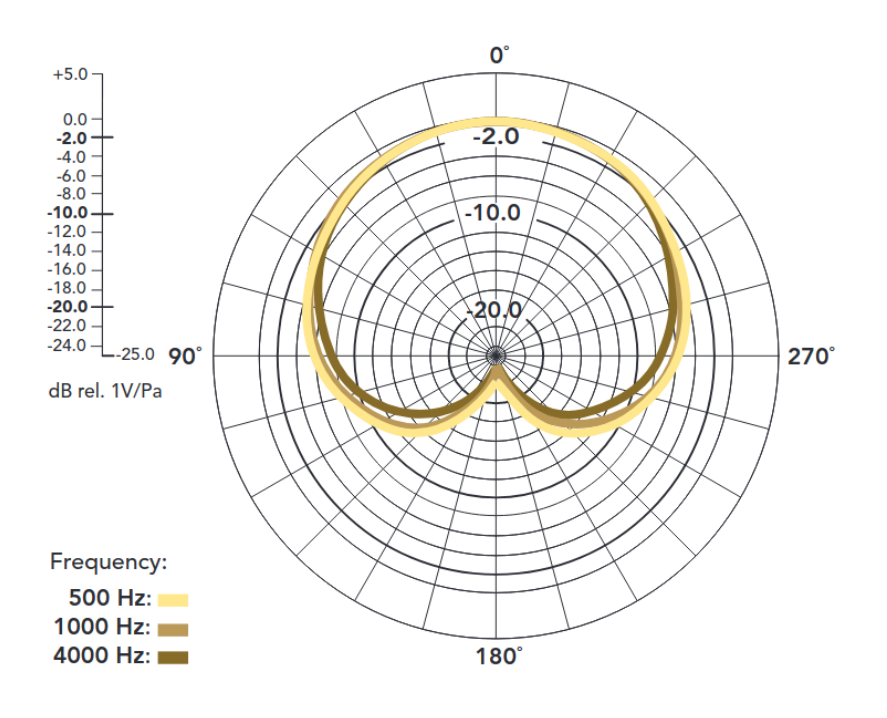
\includegraphics[width=14cm]{Z_anexos_img/rode-nt-polar.png}
\caption{Diagrama polar de la respuesta espacial.}
\label{fig:figure1}
\end{figure}


La respuesta de frecuencias del micrófono por otra parte es mayormente plana, lo que es algo positivo si esperamos una reproducción fiel de la señal original una vez digitalizada.

\begin{figure}[H]
\centering
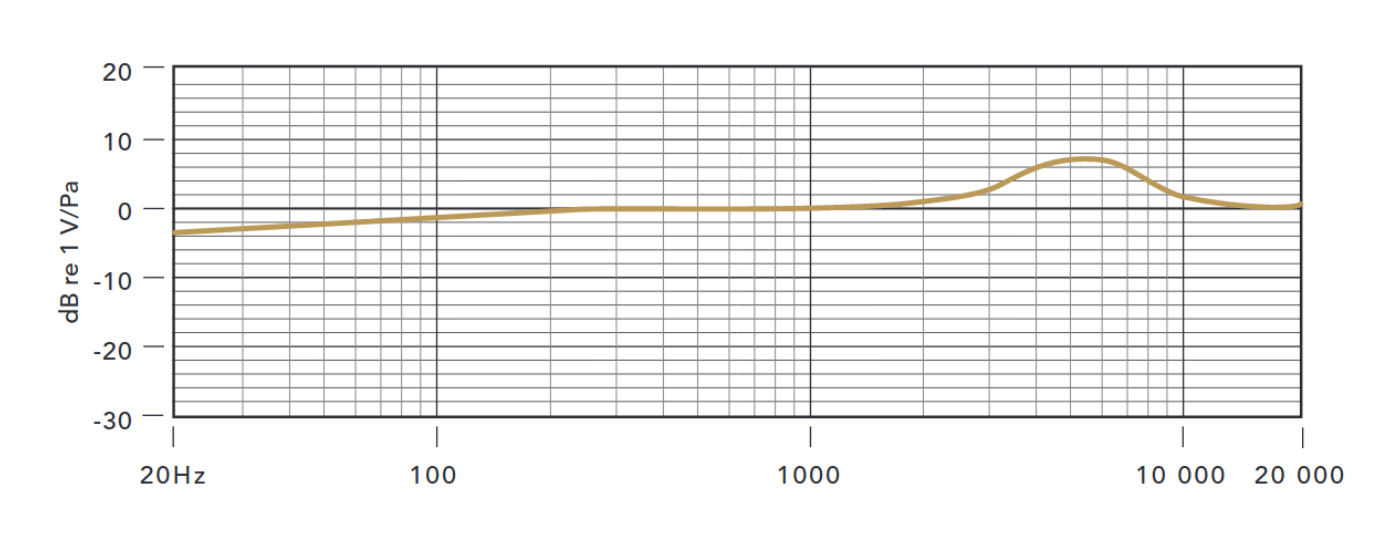
\includegraphics[width=14cm]{Z_anexos_img/rode-nt-response.png}
\caption{Diagrama de respuesta de frecuencias.}
\label{fig:figure1}
\end{figure}

\subsubsection{Software}

No se identificó ningún software específico para la grabación y gestión de datasets de audio, por lo menos no que fuese adecuado para la simple grabación de clips a partir de textos de partida. Se decidió implementar una aplicación simple que tomase una entrada de texto, la segmentase en frases y las presentase al hablante para su grabación de la forma más sencilla posible.

La interfaz es la habitual en una consola de comandos, puesto que era una herramienta para uso exclusivo de la investigación y no sería un producto final para otros usuarios no se consideró ofrecer una interfaz mejor.

\begin{figure}[H]
\centering
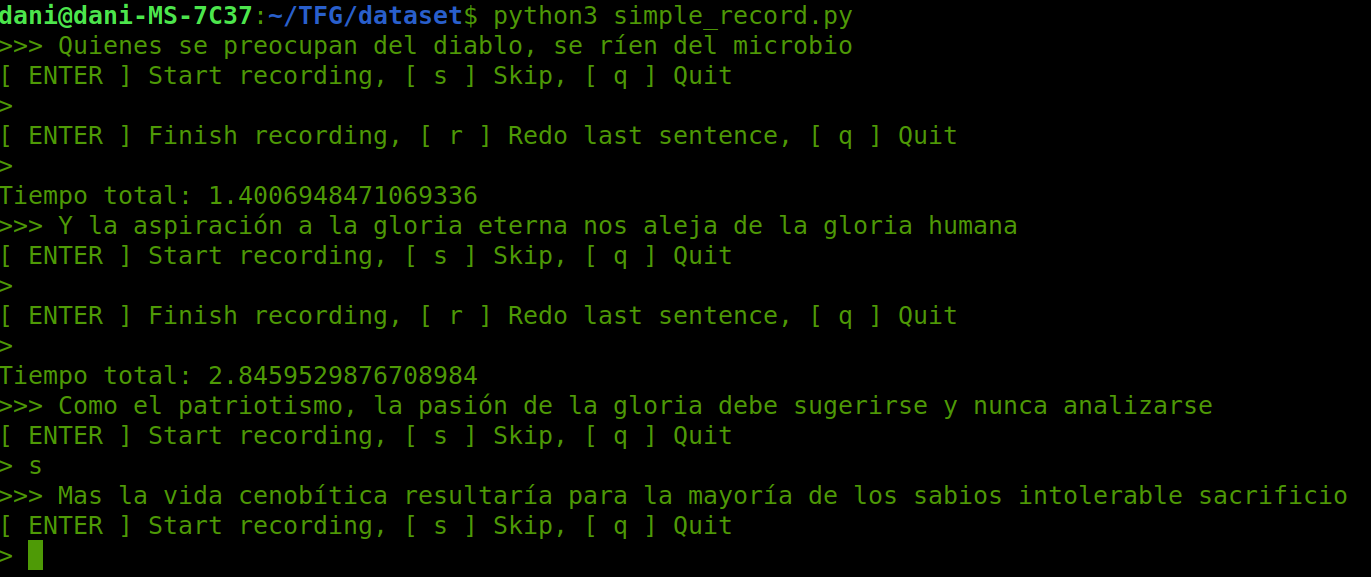
\includegraphics[width=14cm]{Z_anexos_img/record-0.png}
\caption{Interfaz de consola con la que se generó el dataset de audio.}
\label{fig:figure1}
\end{figure}

El funcionamiento es muy simple, cada frase a grabar se muestra por pantalla, el inicio de la grabación comienza cuando se pulsa ENTER y finaliza igualmente cuando se pulsa ENTER. Si ha habido algún error de grabación se puede repetir la última frase grabada y si el texto por el motivo que sea se considera inadecuado para el dataset se puede saltar a la siguiente frase.

Por ejemplo, para el caso base que queremos entrenar se han ignorado nombres propios y términos que no siguen las reglas propias de pronunciación del castellano. Excluimos esencialmente extranjerismos. 

El programa graba cada fragmento como un fichero .wav separado, bien con la calidad original de grabación o bien con algún procesamiento o modificación. Al mismo tiempo se registra en un fichero una nueva entrada que contiene la ruta al fichero de audio y el fragmento de texto.

Este será el formato del dataset final, se ha empleado una barra vertical para separar los campos del fichero porque es el formato original del dataset LJSpeech y es más rápido adaptar modelos ya existentes.

\subsubsection{Reducción de ruido}

Por mucho que se intentó encontrar el ambiente más apartado de ventanas y otros sonidos ambientales fue imposible eliminar del todo el ruido de las muestras simplemente grabadas. 

Para postprocesar los ficheros de sonido y reducir aún más la cantidad de ruido base en el dataset se probaron diferentes herramientas de edición de sonido.

Audacity es un programa de edición de audio bastante conocido y es software libre, entre las diferentes herramientas de manipulación de sonido que tiene se encuentra un reductor de ruido\footnote{Más información en \url{https://manual.audacityteam.org/man/noise_reduction.html}}. Su funcionamiento consiste en seleccionar una muestra que contenga únicamente ruido, de donde el programa extraerá las frecuencias que deberá reducir en el resto de la señal.

Esta forma de reducir el ruido funciona bien cuando el ruido es constante, pero no en el caso de ruidos que puedan variar en el tiempo ni especialmente puntuales\footnote{Su propia documentación así lo indica: «It is not suitable for individual clicks and pops, or irregular background noise such as from traffic or an audience»}.

La segunda opción que se barajó fue emplear un filtro del proyecto Xiph denominado RNNoise\footnote{\url{https://github.com/xiph/rnnoise}}, que ha sido entrenado con muestras reales de ruido y para el que tenemos modelos\footnote{\url{https://github.com/GregorR/rnnoise-models}} específicamente entrenados para el procesamiento de voz.

Esta fue la forma en la que finalmente se procesaron todas las muestras de audio por demostrar ofrecer los mejores resultados frente a las diferentes fuentes de ruido.

[Ejemplo de uso con ffmpeg]

\newpage 
\subsection{Entrenamiento en Google Colab}
\label{Entrenamiento en Google Colab}

Aunque la mayor parte de los entrenamientos se han realizado en local empleando hardware propio, en cierto momento se consideró que podía ser adecuado realizar más de un entrenamiento de manera simultánea.

El precio actual de las GPUs volvía esto imposible si se quería seguir trabajando simplemente en local, por lo que se exploraron las diferentes opciones posibles y su coste.

Google Colab es ahora mismo la opción más económica para el entrenamiento de modelos que requieran del uso intensivo de GPU. Existen dos rangos de precios: en el primer caso por 10€ se accede a una cuenta Colab Pro, en el segundo caso por 50€ al mes se obtiene una cuenta Colab Pro +.

Google es intencionalmente poco preciso sobre los derechos y recursos a los que se puede acceder en ambos casos, pero la experiencia de los usuarios indica que los recursos de hardware no están asegurados y simplemente se reparten entre los usuarios. Este reparto es una cola con prioridades donde los usuarios Pro + tiene preferencia.

Google Colab esencialmente proporciona acceso a GPUs Nvidia P100 (PCIe) y aceleradores Nvidia T4, en nuestro caso suficiente para los entrenamientos pero algo más lento que el entrenamiento en local.

\begin{figure}[H]
\centering
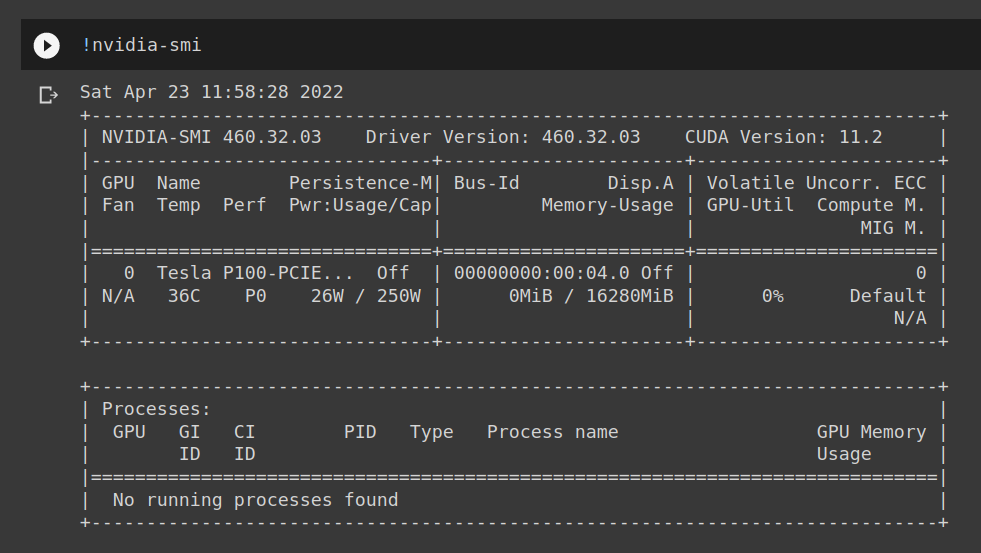
\includegraphics[width=14cm]{Z_anexos_img/colab-1.png}
\caption{Ejemplo de GPU asignada a una instancia de Google Colab Pro +.}
\label{fig:figure1}
\end{figure}

El problema esencial de Google Colab es que su diseño no está orientado al funcionamiento en sesiones largas, sea cual sea el tipo de cuenta que uno tenga. En el caso de cuentas Pro + se asegura un máximo de 24h de duración de las sesiones, en las cuentas Pro y gratuitas es notablemente menor.

Para poder sortear este problema se elaboraron una serie de herramientas que permitían reanudar el entrenamiento tras el fin de la sesión de forma rápida y conservando en todo momento el progreso del entrenamiento. Los notebooks de Colab se ejecutan en un entorno virtualizado que se elimina una vez finaliza la sesión por lo que todos los datos se pierden de otra forma.

Un ejemplo de notebook de Colab empleado se puede consultar aquí: \url{https://colab.research.google.com/drive/1ph_y84bRc-hKtFhmI4tDAiOZpm-LQuUn}

El conjunto de scripts empleados para entrenar, subir los resultados parciales a una instancia de NextCloud y reanudar los entrenamientos se encuentran en este repositorio: \url{https://github.com/daniel-dona/TFG-colab-train-helpers}

De forma resumida, el funcionamiento del notebook es el siguiente:

\begin{enumerate}
    \item Descarga de datasets y herramientas
    \item Descarga del último checkpoint guardado
    \item Inicio o continuación del entrenamiento
    \item Lanzamiento en segundo plano de un proceso que suba el último checkpoint a un almacenamiento remoto
\end{enumerate}

Este mecanismo se empleó para entrenar varios modelos con el dataset LJSpeech, especialmente las primeras pruebas con el modelo VITS.

\newpage 
\subsection{Análisis de datasets}
\label{Análisis de datasets}

Prácticamente la totalidad de modelos estudiados usan el dataset LJSpeech \hyperref[AX_1]{[23]} como referencia. Este modelo grabado a partir de una única hablante se caracteriza por su alta calidad y su tono neutro.

El dataset contiene un total de 13100 clips de audio, con un total de 225715 palabras. Contiene aproximadamente 24 horas de grabación en total y los clips de sonido oscilan entre los 2 segundos y los 10 segundos.

Para nuestras pruebas nos interesaba especialmente estudiar no tanto el dataset propiamente sino el resultado de convertirlo a fonemas con algunas de las herramientas (entrenadas o paramétricas) que nuestro toolkit incluía. 

Aunque es posible entrenar los modelos directamente a partir de caracteres y dejar que los mecanismos de atención del modelo encuentren las diferencias fonéticas del lenguaje a partir de los caracteres anteriores y siguientes, se suelen emplear conversores a fonemas en la mayoría de modelos por hacer más rápido el aprendizaje.

En primer lugar analizamos la presencia estadística de los fonemas empleando un histograma:

\begin{figure}[H]
\centering
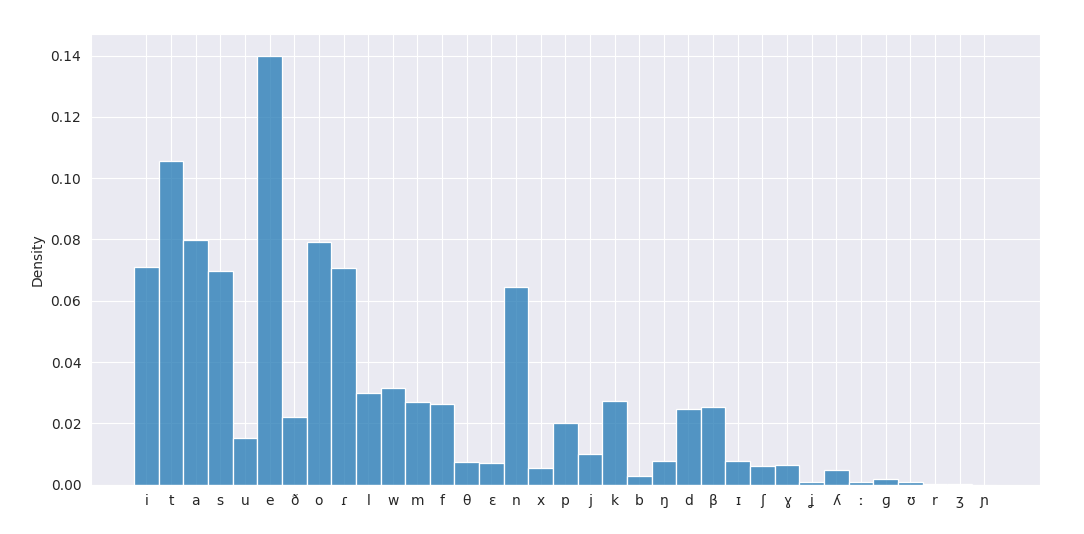
\includegraphics[width=14cm]{Z_anexos_img/ljs-1.png}
\caption{Histogramas de fonemas en LJSpeech}
\label{fig:figure1}
\end{figure}

Aunque ciertos fonemas se encuentran claramente infrarepresentados en el dataset, el tamaño del propio dataset nos permite ignorar esto. 

Sabíamos que algunos modelos paramétricos empleaban no fonemas, sino parejas de fonemas para representar la unidad básica para la síntesis de voz. Por ello decidimos además analizar la presencia de ciertas parejas de fonemas.

\begin{figure}[H]
\centering
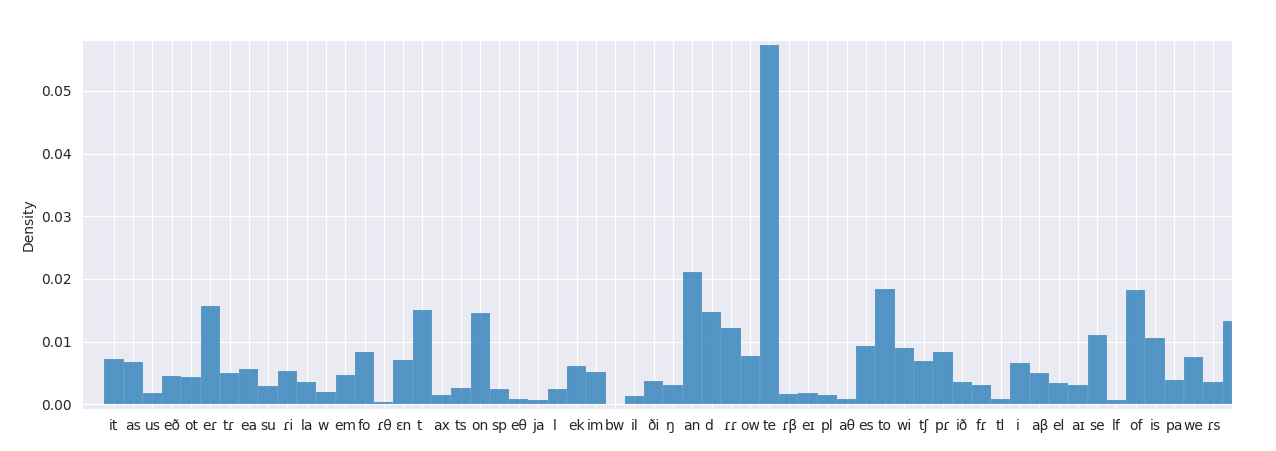
\includegraphics[width=14cm]{Z_anexos_img/ljs-2.png}
\caption{Histogramas de pares de fonemas en LJSpeech (más frecuentes).}
\label{fig:figure1}
\end{figure}

\begin{figure}[H]
\centering
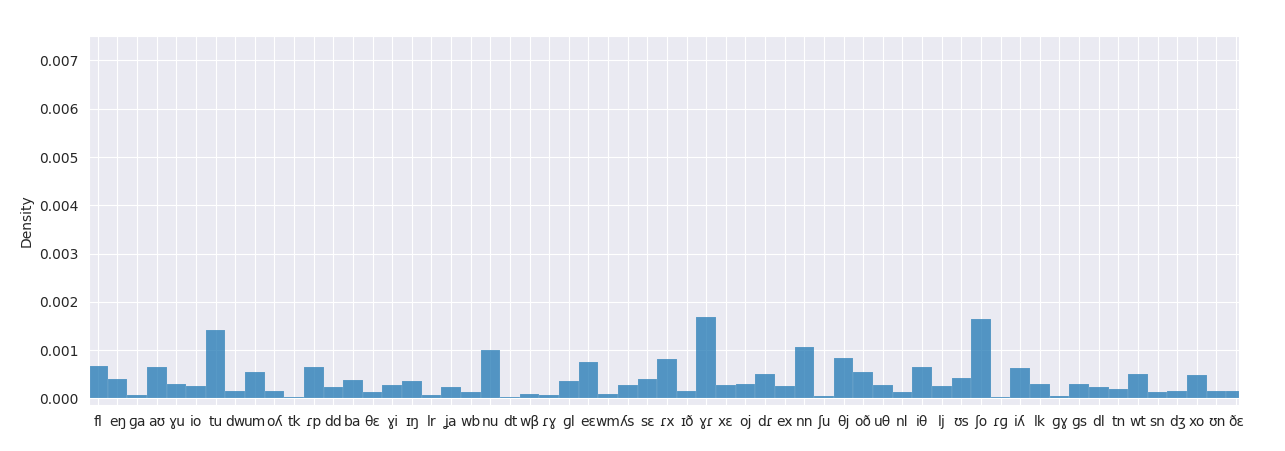
\includegraphics[width=14cm]{Z_anexos_img/ljs-3.png}
\caption{Histogramas de pares de fonemas en LJSpeech (menos frecuentes).}
\label{fig:figure1}
\end{figure}



En este caso encontramos que ciertas parejas de fonemas aparecen de forma muy muy escasa en el dataset. De la misma forma que ciertos grafemas son mucho más comunes que otros en una lengua, es esperable que ciertos fonemas y parejas de fonemas sean raros igualmente.

Sabemos que este dataset es el más empleado por ofrecer unos buenos resultados en inglés, por lo que podemos asumir que la inmensa mayoría de combinaciones fonéticas están cubiertas. 

Sabiendo que nosotros no podemos aspirar a un dataset tan grande, esta distribución de los datos puede suponer que con un dataset pequeño ciertas palabras se sinteticen con notablemente peor calidad que otras o que directamente el modelo no haya sido entrenado con un fonema que aparezca en una inferencia determinada.

Esto último también puede suceder si se intenta inferir a partir de un texto/fonemas de un idioma distinto o una variedad dialectal distinta.

\newpage 
\subsection{Entorno de entrenamiento}
\label{Entorno de entrenamiento}

Con anterioridad se han comentado las dificultades para realizar entrenamientos largos empleando Google Colab, es por ello que se relegó a un segundo plano como entorno para realizar este tipo de tareas. El entorno principal para el entrenamiento fue en su lugar un computador propio con la siguiente configuración de hardware:

\begin{itemize}
    \item CPU: AMD Ryzen 9 5900X (12 cores/24 threads)
    \item Main memory: DDR4 3600 CL18 (32 GB)
    \item GPU: Nvidia RTX3080 Ti (12 GB), 10240 CUDA cores
    \item Disco: NVMe WD 1TB SN500 
\end{itemize}

El sistema operativo base en el que se han desarrollado los entrenamientos es Ubuntu 20.04, siendo la versión de Python 3 propia de la distribución la 3.8.10.

Los drivers de NVIDIA que habilitaron poder emplear aceleración mediante CUDA fueron los 510.47.03. 

NVIDIA emplea un concepto denominado Compute Capability para identificar características entre las diferentes generaciones de aceleradores y tarjetas gráficas. La versión de esta tarjeta gráfica es la 8.6, también identificada en algunas librerías como SM\_86.

Además los drivers de NVIDIA específicamente para CUDA tienen diferentes versiones, siendo los más recientes la versión CUDA 11.6. Esta versión, junto a la Compute Capability tiene que ser compatible con las diferentes librerías que quieran hacer uso de la GPU para acelerar cálculos.

En el caso de Torch, la librería principal para los entrenamientos, se tuvo que instalar una versión específica para poder hacer uso de los recursos de computación disponibles.

\begin{lstlisting}
python3 -m pip install torch==1.10.2+cu113 torchvision==0.11.3+cu113 torchaudio==0.10.2+cu113 -f https://download.pytorch.org/whl/cu113/torch_stable.html
\end{lstlisting}

Durante los entrenamientos el uso de la tarjeta gráfica supone un consumo de energía de aproximadamente 300W adicionales al consumo del resto del sistema, esto supone una gran cantidad de calor que puede ser problemático para la vida útil de los componentes electrónicos.

\begin{figure}[H]
\centering
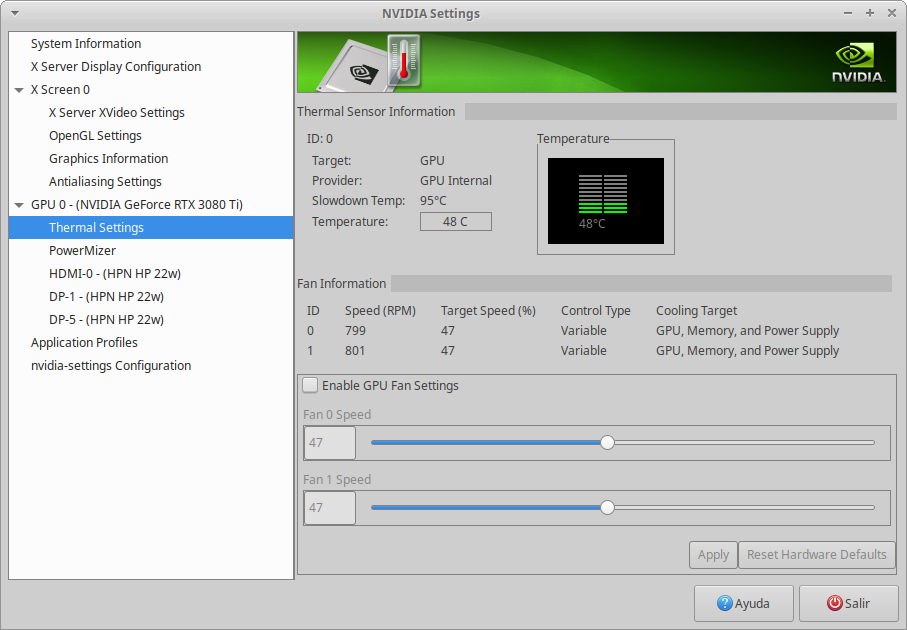
\includegraphics[width=14cm]{Z_anexos_img/nvidia-smi.png}
\caption{Interfaz de gestión de NVIDIA en Linux.}
\label{fig:figure1}
\end{figure}

Para mantener el hardware en una zona segura, se ha forzado manualmente el uso intensivo de los ventiladores de la tarjeta gráfica para bajar lo máximo posible la temperatura. Esto en algunos momentos ha sido conflictivo con las labores de grabación del dataset de voz al generar bastante ruido.